\lecdate{20.03.2017}
Problem: Aussagenlogik ist wenig mächtig.\\
Aussagen, die sich nicht formulieren lassen:
\begin{itemize}
\item „Alle Vögel können fliegen.“\\
(Nur formulierbar, wenn alle Vögel einzeln als Atomformeln beschrieben werden. Diese Formel der Aussagenlogik wäre dann allerdings sehr lang.)
\item „Wenn X eine Katze ist, dann ist X ein Haustier.“\\
(In der Aussagenlogik sind keine Variablen möglich.)
\item „Für jedes Land gibt es eine Hauptstadt.“
\end{itemize}

\section{Syntax der Prädikatenlogik}
\cparagraph{Definition}
Sei $V$ eine Menge von Variablen, $K$ eine Menge von Konstante und $F$ eine Menge von Funktionssymbolen.
\begin{itemize}
\item Dann sind alle Variablen $V$ und Konstanten in $K$ Terme.
\item Wenn $t_1, \dots, t_n$ Terme sind und $f$ ein $n$-stelliges Funktionssymbol ist, dann ist auch $f(t_1, \dots, t_n)$ ein Term. 
\end{itemize}

\cparagraph{Beispiel}
$V=\{x,y,z\},\; K=\{a,b,c\},\; F=\{+,*\}$. Terme sind $x,a,x+a,x*(x+1)$.

\cparagraph{Definition}
Sei eine Menge von Prädikatensymbolen gegeben. Die Formeln der Prädikatenlogik sind induktiv definiert:
\begin{itemize}
\item Wenn $t_1, \dots, t_n$ Term und $P$ ein Prädikatensymbol der Stelligkeit $n$ ist, dann ist $P(t_1, \dots, t_n)$ eine Formel.
\item Sind $F,G$ Formeln, dann auch $F\wedge G, \; F\vee G,\; \neg F,\; (F)$.
\item Wenn $x$ eine Variable und $F$ eine Formel ist, dann sind auch $\forall x \,F, \; \exists x\,F$ Formeln.
\end{itemize}

\cparagraph{Bemerkung} Wie in der Aussagenlogik definiert sich $\to, \; \leftrightarrow$.\\
Vorrang der Operatoren: $\neg;\; \forall, \; \exists;\; \wedge, \; \vee;\; \to,\; \leftrightarrow$

\cparagraph{Beispiel}
\begin{itemize}
\item $\forall x\, (vogel(x) \to fliegt(x))$\\
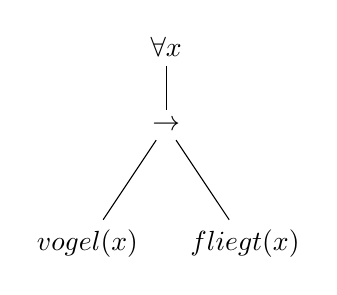
\begin{tikzpicture}
\node (v1) at (-0.5,2) {$\forall x$};
\node (v2) at (-0.5,1) {$\to$};
\node (v3) at (-1.5,-0.5) {$vogel(x)$};
\node (v4) at (0.5,-0.5) {$fliegt(x)$};
\draw (v1) -- (v2);
\draw (v2) -- (v3);
\draw (v2) -- (v4);
\end{tikzpicture}
\item $\forall x\, (katze(x) \to haustier(x))$
\item $\forall x\, (land(x) \to \exists y\, hauptstadt (x,y))$\\
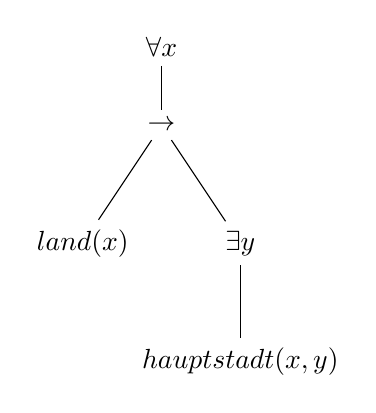
\begin{tikzpicture}
\node (v1) at (-0.5,2) {$\forall x$};
\node (v2) at (-0.5,1) {$\to$};
\node (v3) at (-1.5,-0.5) {$land(x)$};
\node (v4) at (0.5,-0.5) {$\exists y$};
\draw (v1) -- (v2);
\draw (v2) -- (v3);
\draw (v2) -- (v4);
\node (v5) at (0.5,-2) {$hauptstadt(x,y)$};
\draw (v4) -- (v5);
\end{tikzpicture}
\item $katz(feli)$ mit $feli \in K$
\end{itemize}

\section{Semantik der Prädikatenlogik (informal)}
Wir betrachten zunächst eine (unwichtige) Menge $U$ (Universum), die alle zu betrachtenden Objekte (Vögel, Katzen, Länder usw.) enthält. Davon betrachten wir Teilmengen, z.B. die Menge aller Vögel, Länder usw. sowie mehrstellige Relationen auf $U$ (z.B. Hauptstadt, verheiratet).

Beispiel: $Hauptstadt=\{(Berlin,\;Deutschland), (Paris, \; Frankreich)\} \subseteq \underbrace{U \times U}_{oder:\; Stadt\times Land}$\\
Den Prädikatensymbolen müssen Prädikate (Relationen) zugeordnet werden.

Beispiel: Ordnen dem Prädikatensymbol $vogel$ das Prädikat „Menge aller Vögel“ zu.\\
Dadurch ergibt sich der Wahrheitswert einer Formel: 
\begin{itemize}
\item Die Formel $P(t_1, \dots, t_n)$ ist wahr \gdw{} $(t_1, \dots, t_n) \in P$.
\item Die Wahrheit von $F\wedge G, \; F\vee G,\; \neg F$ ist wie in der Aussagenlogik definiert.
\item $\exists x \, F$ ist wahr \gdw{} es ein $x$ aus dem Universum gibt, mit dem $F$ wahr ist.
\item $\forall x \, F$ ist wahr \gdw{} $F$ für alle $x$ aus dem Universum wahr ist.
\end{itemize}
\cparagraph{Beispiel}
Sei $vogel=\{Amsel, Drossel, Fink, Star\}$ und $fliegt=vogel \cup \{Maikaefer, A380\}$
\begin{itemize}
\item $vogel(Amsel)$ ist wahr.
\item $vogel(Maikaefer)$ ist falsch.
\item $\exists x \, vogel(x)$ ist wahr.
\item $\forall x \, vogel(x)$ ist falsch.
\item $\forall x \,(vogel(x) \to fliegt(x))$ ist wahr.
\end{itemize}

\cparagraph{Beispiel} Sei $land=\{Deutschland, Frankreich\}$ und \\
$hauptstadt = \{ (Berlin, Deutschland), (Paris, Frankreich) \}$.\\
Für jedes Land gibt es eine Hauptstadt:\\
$\forall x \,(land(x)\to \exists y \, hauptstadt(y,x))$







